\subsection{How does agent degradation compare to repository histories?}
\label{sec:agent-vs-human}

\begin{figure}[t]
    \centering
    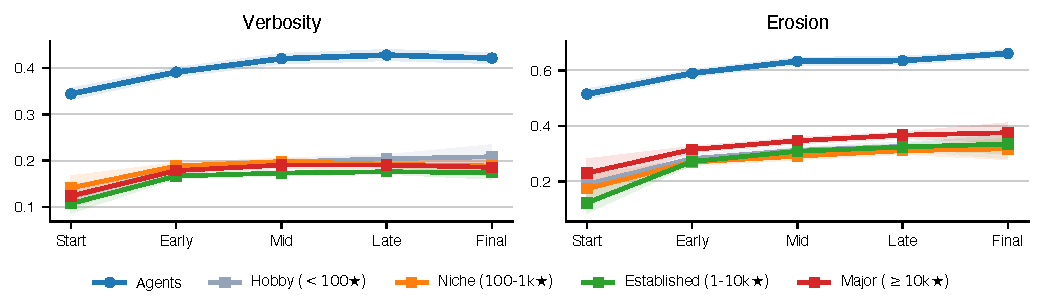
\includegraphics[width=\linewidth]{figures/agent_human_trajectory.pdf}
    \caption{\textbf{Agents produce lower quality code and degrade it faster than real developers.} Verbosity and erosion across normalized trajectory progress, with 95\% confidence intervals. GitHub-star bins over \avhPanelN{} repositories for a total of $\avhTemporalCkpts$ checkpoints. \autoref{tab:agent-vs-human} has HEAD commit details.}
    \label{fig:agent-human-trajectory}
\end{figure}

To answer this, we collect \avhPanelN{} Python repositories ranging from hobby projects under 100 stars to major frameworks with over 10k stars and 2M LOC, covering web frameworks, scientific computing, infrastructure, and utilities. For each repository, we randomly sample up to 30 source-modifying commits totaling \avhTemporalCkpts{} commits. We treat each repository's most recent commit at the time of collection as its current state for cross-sectional comparisons and the full commit sequence as analogous to an agent trajectory.

\autoref{fig:agent-human-trajectory} shows the human panel averages 0.19 verbosity and 0.34 erosion. Agent checkpoints sit \avhAllVerbRatio{}$\times$ and \avhAllErosionRatio{}$\times$ above those means. Only \avhHumanAboveAgentVerbN{} of \avhPanelN{} repositories cross the agent verbosity mean. Agent verbosity grows by \avhAgentVerbSlopeMedian{} per checkpoint and erosion by \avhAgentErosSlopeMedian{}; the human medians are \avhHumanVerbSlopeMedian{} and \avhHumanErosSlopeMedian{}. Inside the iteration loop, agents accumulate verbosity roughly 7$\times$ faster and erosion 5$\times$ faster. Erosion rises in \erosionPctIncreasing{}\% of agent trajectories against \avhTemporalErosRisingPct{}\% of human repositories.

\begin{table}[t]
    \centering
    \caption{Verbosity and erosion at HEAD commit, by GitHub-star tier and against agent checkpoints.}
    \label{tab:agent-vs-human}
    \footnotesize
    \setlength{\tabcolsep}{6pt}
    \begin{tabular}{lccc}
        \toprule
        Group & $n$ & Verbosity & Erosion \\
        \midrule
        Hobby ($< 100\bigstar$) & 114 & $0.21 \pm 0.14$ & $0.33 \pm 0.25$ \\
        Niche ($100\text{--}1\text{k}\bigstar$) & 124 & $0.19 \pm 0.11$ & $0.32 \pm 0.22$ \\
        Established ($1\text{k}\text{--}10\text{k}\bigstar$) & 120 & $0.18 \pm 0.08$ & $0.33 \pm 0.20$ \\
        Major ($\geq 10\text{k}\bigstar$) & 115 & $0.19 \pm 0.10$ & $0.37 \pm 0.19$ \\
        \midrule
        Human panel (all) & 473 & $0.19 \pm 0.11$ & $0.34 \pm 0.22$ \\
        Agent checkpoints & 2869 & $0.44 \pm 0.18$ & $0.68 \pm 0.20$ \\
        \bottomrule
    \end{tabular}
\end{table}


For the \avhAgentEraBothN{} repositories with at least three commits in each of the pre- and post-January-2024 windows, within-repository medians shift by $+\avhAgentEraVerbShiftMedian$ for verbosity and $+\avhAgentEraErosShiftMedian$ for erosion; \avhAgentEraErosHigherPct{}\% of these repositories are more eroded after 2024 than before. The shift is consistent with a small uptick in human-authored slop after agent assistance became common, and it remains far below what an agent accumulates in a single checkpoint. \autoref{sec:human-repo-panel} extends this analysis. 
    